\chapter{Numerical Methods and Implementation Details}\label{ch:methods}

The implementation consists of two finite-element applications coupled through
one neural network. Offline, NGSolve solves periodic RVEs and stores energy,
stress and tangent; PyTorch trains the network on these data. Online, the trained
network is evaluated at every quadrature point of a macroscopic NGSolve model and
supplies stress and tangent to Newton's method.

\section{Choice of language and libraries}

The code is written in Python~3.11. This lets a single language host both the
finite-element library NGSolve~\cite{Schoeberl2014} (C++ core, Python front end,
symbolic differentiation of variational forms) and PyTorch~\cite{Paszke2019}
(reverse-mode automatic differentiation, optimizers). Python's overhead is
confined to orchestration. All heavy kernels run in compiled code: sparse
assembly and direct solvers in NGSolve, and batched tensor algebra in PyTorch.
NumPy handles array exchange; Matplotlib is used for plotting. All computations
use double precision.

\section{Phase 1: the PyTorch--NGSolve material bridge}\label{sec:bridge}

NGSolve has no hook for a constitutive law written in an external framework.
The bridge (\code{src\slash{}ngsolve\_umat.py}) therefore passes data through
\code{IntegrationRuleSpace} grid functions. These store one value per
quadrature point and are tied to a fixed integration rule. Each Newton
iteration performs the following steps (routine \code{assemble\_system}):
\begin{enumerate}
  \item interpolate $\F=\Iten+\nabla\bm u$ into a nine-component quadrature-point
        function and gather it as an array of shape $(n_q,3,3)$;
  \item reject non-finite values and any $J\le10^{-8}$ before calling the network;
  \item evaluate $\widehat\Psi$, $\Pstress=\partial\widehat\Psi/\partial\F$ and the nine rows of
        $\Aten=\partial\Pstress/\partial\F$ by repeated reverse-mode AD
        (\code{stress\_and\_tangent});
  \item write $\Pstress$ (9 components) and $\Aten$ (81 components, row-major
        $3i+J$) back into quadrature-point functions;
  \item assemble the residual and the consistent stiffness
        \begin{equation}
          R_a=\int_{\Omega_0}P_{iJ}\,N_{a,i,J}\dd V,\qquad
          K_{ab}=\int_{\Omega_0}N_{a,i,J}\,\Aten_{iJkL}\,N_{b,k,L}\dd V
        \end{equation}
        using \emph{the same} integration rule, and solve for the update on the
        free degrees of freedom.
\end{enumerate}
\textbf{Tricky aspects.} (i) If the residual or stiffness forms were integrated
with a rule other than the one attached to the quadrature-point space, the
material data would be evaluated at the wrong locations. NGSolve raises no error
in that case; the Newton iteration simply loses its quadratic rate. (ii) A
transposed index map or a $6\times6$ shortcut assembles the stiffness of a
different material; V3--V6 detect both. (iii) The tangent needs nine
backward passes through a graph created with \code{create\_graph=True}. This is
the dominant cost of the bridge (\cref{ch:performance}).

\section{Phase 2: periodic RVE solver}

\paragraph{Geometry and periodicity.} The cube with a spherical cavity is built
with Netgen's OCC kernel~\cite{Schoeberl1997}. Opposite faces are identified \emph{before} meshing, so
the surface meshes match node by node, and NGSolve's \code{Periodic} wrapper
shares the corresponding degrees of freedom~\cite{NGSolvePeriodic}. The unknown
is the fluctuation $\bm w$ of \cref{eq:kin}; periodicity therefore applies to $\bm w$
and not to the affine part of the displacement.

\paragraph{Mixed matrix.} The residual of \cref{eq:mixed} is discretized with
Taylor--Hood elements: $P_2$ displacement and $P_1$ pressure. This choice
satisfies the inf--sup condition~\cite{Boffi2013} and avoids the volumetric locking of a
displacement-only low-order discretization at $\kappa/\mu=10^4$~\cite{Simo1985}.
NGSolve differentiates the symbolic residual to give the exact Jacobian. The
production setting uses $h=0.22$ and integration order~10.

\paragraph{Rigid particle and free rotation.} The cavity boundary is a Dirichlet
boundary of the displacement space whose prescribed trace is the exact rigid map
\cref{eq:rigid}. The particle therefore has no deformational degrees of freedom
and no penalty parameter is needed. The three rotation coordinates are found in
an outer Newton loop (\code{src\slash{}free\_particle.py}):
\begin{enumerate}
  \item for the current $\Rten$, solve the mixed periodic RVE by Newton's method (tolerance $10^{-8}$ in production, $10^{-10}$ in the tests);
  \item assemble the resultant moment $\bm m$ of the reactions on the particle;
  \item compute the exact condensed rotational Hessian $\partial\bm m/\partial\bm\theta$
        by one sparse factorization and three sensitivity solves;
  \item update multiplicatively, $\Rten\leftarrow\exp([\delta\bm\theta]_\times)\Rten$
        (Rodrigues' formula), until the moment residual is below $10^{-9}$.
\end{enumerate}
Large or strongly compressive loads start from the identity and are approached
by adaptive load continuation with previous-state or secant predictors.

\paragraph{Homogenization and tangent.} The homogenized energy is the
equilibrated potential divided by $|\Omega|$. The stress is evaluated with
\cref{eq:hm}, adding the matrix stress integral and the work of the full
assembled reaction vector in the nine macroscopic modes. For the tangent, nine
global \code{NumberSpace} unknowns, plus three for the rotation, are appended to
the mixed space. The Hessian of the extended energy is assembled once, the
internal block is factorized once, and \cref{eq:schur} is evaluated with nine
sensitivity solves. No dense inverse is formed and no RVE is re-solved.

\paragraph{Microscale setup.} \Cref{fig:rvesetup} shows the RVE mesh and its boundary
conditions, and \cref{tab:micro} summarizes the production settings of the RVE
computations.

\begin{figure}[htbp]
\centering
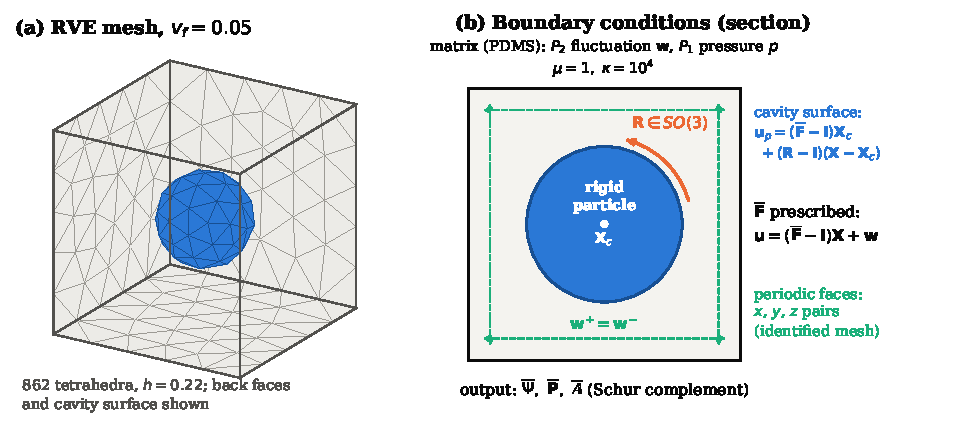
\includegraphics[width=\textwidth]{fig_rve_setup.pdf}
\caption[RVE finite-element model]{RVE finite-element model. (a) Netgen mesh of the matrix for $\vfrac=0.05$; the
particle is not meshed, only its cavity surface (blue) carries the rigid trace. Back
faces shown; opposite faces have identical surface meshes. (b) Section through the
RVE: periodic fluctuation $\bm w$ on all three face pairs, exact rigid motion of the
cavity surface with rotation $\Rten$ from moment equilibrium, and macroscopic
deformation $\Fbar$ imposed through \cref{eq:kin}.}
\label{fig:rvesetup}
\end{figure}

{\small
\begin{xltabular}{\textwidth}{@{}p{3.6cm}X@{}}
\caption{Microscale (RVE) finite-element setup used for all datasets.}\label{tab:micro}\\
\toprule
Item & Setting\\
\midrule
\endfirsthead
\caption[]{\emph{(continued)}}\\
\toprule
Item & Setting\\
\midrule
\endhead
\bottomrule
\endfoot
Domain & unit cube $[0,1]^3$ with centred spherical cavity, radius $r=(3\vfrac/4\pi)^{1/3}$ (0.168, 0.229, 0.288)\\
Geometry and mesh & Netgen OCC kernel, opposite faces identified before meshing; unstructured tetrahedra, $h=0.22$; boundaries \code{xmin}, \dots, \code{zmax}, \code{particle}\\
Mesh size per $\vfrac$ & 1441 / 862 / 875 tetrahedra for $\vfrac=0.02/0.05/0.10$\\
Elements & Taylor--Hood: $P_2$ periodic vector displacement fluctuation, $P_1$ periodic pressure\\
Degrees of freedom & 7518 / 5043 / 5102 in total, 5654 / 3275 / 3310 free after periodic and rigid-trace constraints; plus 3 rotation unknowns\\
Quadrature & integration order 10 in all volume and surface forms\\
Matrix material & mixed near-incompressible neo-Hookean, \cref{eq:mixed}: $\mu=1$, $\kappa=10^4$\\
Particle & exactly rigid: Dirichlet trace \cref{eq:rigid} on \code{particle}; free rotation from moment equilibrium\\
Kinematic loading & prescribed $\Fbar$ through $\F=\Fbar+\nabla\bm w$; translation gauge fixed\\
Nonlinear solver & Newton with exact symbolic Jacobian and backtracking line search with $J>0$ check; tolerance $10^{-8}$ (residual), $10^{-9}$ (moment); adaptive load continuation\\
Linear solver & sparse direct factorization (UMFPACK~\cite{Davis2004})\\
Homogenized tangent & 9 macroscopic + 3 rotational \code{NumberSpace} unknowns; one factorization, Schur complement \cref{eq:schur}\\
\end{xltabular}
}

\paragraph{Mesh and quadrature convergence.} The production resolution was chosen by
a convergence study (\code{rve\_phase2\_convergence.json}) before any dataset was
generated. Eight macroscopic states (hydrostatic tension and compression, uniaxial
and biaxial tension, simple shear, a combined non-symmetric state and two boundary
states of the sampling domain) were solved at $\vfrac=0.02$ and $0.10$ on three
meshes ($h=0.30$, $0.22$, $0.16$) with integration orders 6 and 10. Energy, stress
and tangent were compared with the finest solution ($h=0.16$, order~10), and
accuracy targets of $0.2\,\%$, $0.5\,\%$ and $1\,\%$ were set in advance.
\Cref{fig:rveconv} gives the largest error over the eight states. The coarse mesh
misses the energy and stress targets for simple shear at $\vfrac=0.10$
($7.1\times10^{-3}$ and $7.5\times10^{-3}$); $h=0.22$ satisfies all targets, the energy target with a
margin of a factor of 2.6. At $\vfrac=0.10$ the remaining error of
$7.7\times10^{-4}$ is the same for energy, stress and tangent, for every state and
for both coarser meshes, except for simple shear, whose energy and stress errors at
$h=0.22$ are $5.7\times10^{-4}$ and $7.5\times10^{-4}$. Such a
uniform relative offset points to the polyhedral approximation of the particle
surface, which changes the effective volume fraction slightly, rather than to the
resolution of the displacement field. The integration order has no visible
effect (order~6 versus 10 at $h=0.16$: below $10^{-9}$). Order~10 was nevertheless
kept for production as a conservative choice.

\begin{figure}[htbp]
\centering
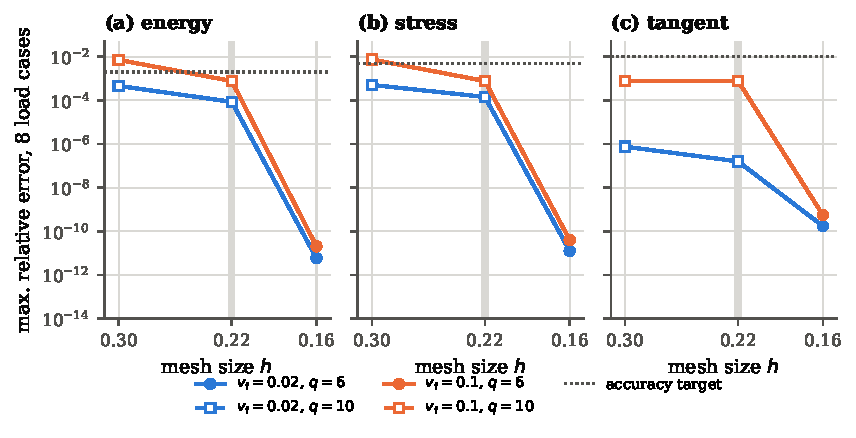
\includegraphics[width=\textwidth]{fig_rve_convergence.pdf}
\caption[RVE mesh and quadrature convergence]{RVE mesh and quadrature convergence: largest relative error of the
homogenized (a) energy, (b) stress and (c) tangent over eight load states, relative
to the solution with $h=0.16$ and integration order~10. Dotted: accuracy target set
before the study. Grey band: production mesh $h=0.22$. Points at $h=0.16$ compare
integration order 6 with 10 only.}
\label{fig:rveconv}
\end{figure}

\section{Dataset generation}

Deformation gradients are drawn by a seeded uniform perturbation of $\Iten$ and
filtered for $J>0$ and a bounded condition number. Targeted campaigns add
stratified compression ($J\in[0.51,0.60]$) and expansion ($J\in[1.50,1.80]$)
states. Every deformation state is solved at all three volume fractions, and the
whole \emph{group} is assigned to the training, validation or test split. This
prevents the same loading from appearing in two splits. A record is accepted
only if the mixed, rotational and condensed residuals are below $10^{-8}$, the
minimum microscopic $J$ exceeds its floor, the particle clearance is positive and
all arrays are finite. Per-sample results are written atomically, so an
interrupted cluster job resumes without trusting partial files. A JSON manifest
records the configuration, schema, software versions, split counts and SHA-256
hashes. \Cref{tab:datasets} lists the datasets.

{\small
\begin{xltabular}{\textwidth}{@{}lrX@{}}
\caption[Direct-RVE datasets]{Direct-RVE datasets (each record: $\Fbar$, $\vfrac$, $\Psibar$, $\Pbar$, $\Abar$, $\Rten$, residuals, diagnostics).}\label{tab:datasets}\\
\toprule
Dataset & Records & Purpose\\
\midrule
\endfirsthead
\caption[]{\emph{(continued)}}\\
\toprule
Dataset & Records & Purpose\\
\midrule
\endhead
\bottomrule
\endfoot
Phase 2 pilot & 300 & first schema; integrity and pipeline test\\
Phase 3 & 900 & intermediate dataset generated before the targeted sets\\
Phase 4 compression & 1080 & compressive states\\
Phase 5 independent & 360 & independently seeded set\\
Phase 6 targeted & 1260 & targeted sampling of the $J$ tails; stage-1 training data\\
Phase 7 independent & 600 & new seed; 531 eligible test records (33 train and 33 validation records of it entered stage~2)\\
Fresh holdout (\code{rve\_extra\_holdout}) & 90 & generated after the checkpoint was frozen; evaluation and timing benchmark\\
Shear adaptation & 33 & simple-shear fine-tuning data (18 train, 6 validation, 9 development test)\\
Shear context holdout & 15 & simple-shear cases used to compare the adaptation variants (\cref{sec:shearvariants})\\
Final shear holdout & 15 & 12 scored simple-shear cases, new microstructure seed\\
\end{xltabular}
}
The ten datasets hold 4653 distinct records. The stage-2 dataset
(\code{rve\_phase6\_phase7\_training}, 1671 records, split 909/225/537) is a composite
drawn from the Phase~6 and Phase~7 sets and adds no further records; the 189 Phase~6
test records are not part of it.

\section{Network architecture}\label{sec:architecture}

\Cref{fig:arch} shows the partially input-convex network implemented in
\code{src/picnn.py}. The deformation gradient enters only through the invariant
features $\bm y=[I_1,\,I_2,\,J,\,-\ln J]$, which makes the energy isotropic and
objective by construction. Features and context are standardized with fixed means
and positive scales from the training split, $\hat{\bm y}=(\bm y-\bm m_y)\oslash\bm s_y$
and $\hat c=(\vfrac-m_c)/s_c$; a positive affine scaling preserves convexity and
monotonicity. With $W^{+}=\mathrm{softplus}(W)$ and $\sigma=\mathrm{softplus}$, the
forward pass is
\begin{align}
  [\bm b_1,\bm b_2,\bm b_3] &= \bm V_2\,\sigma(\bm V_1\hat c+\bm\beta_{c1})+\bm\beta_{c2},\label{eq:ctx}\\
  \bm z_1 &= \sigma\bigl(W_{y,1}^{+}\hat{\bm y}+\bm\beta_1+\bm b_1\bigr),\\
  \bm z_l &= \sigma\bigl(W_{z,l}^{+}\bm z_{l-1}+W_{y,l}^{+}\hat{\bm y}+\bm\beta_l+\bm b_l\bigr),\qquad l=2,3,\\
  \Psi_{\mathrm{raw}} &= \bm w_{\mathrm{out}}^{+}\cdot\bm z_3+\beta_{\mathrm{out}},
\end{align}
followed by the reference normalization \cref{eq:norm}. All weights acting on
$\hat{\bm y}$ or on hidden states are non-negative and $\sigma$ is convex and
non-decreasing, so $\Psi_{\mathrm{raw}}$ is convex and non-decreasing in $\hat{\bm y}$
for every $\vfrac$. The context network \cref{eq:ctx} is unconstrained, because it only
shifts biases. The passthrough connections $W_{y,l}^{+}\hat{\bm y}$ let every layer see
the features directly, as proposed for ICNNs~\cite{Amos2017}. The positive weights
are initialized such that $\mathrm{softplus}(W)\approx0.05$ ($W_y$, $\bm w_{\mathrm{out}}$)
and $0.02$ ($W_z$), which avoids the overly stiff initial energy that
$\mathrm{softplus}(0)\approx0.69$ would produce. Stress and tangent are obtained by
automatic differentiation of $\widehat\Psi$ with respect to $\F$. \Cref{tab:params}
lists all trainable parameters.

\paragraph{How weights and biases are chosen.} None of the 5793 parameters is set by
hand; all are found by the training described in \cref{sec:training}. Only their
starting values and constraints are prescribed. Each constrained weight is stored as an
unconstrained raw value $W$ and enters the network as $\mathrm{softplus}(W)$, so any
raw value yields a non-negative effective weight. The raw values are drawn from a
normal distribution with standard deviation $0.05$ around
$\log(e^{w_0}-1)$, which makes the effective weight start near $w_0=0.05$
($W_y$, $\bm w_{\mathrm{out}}$) or $0.02$ ($W_z$). The biases $\bm\beta_{1..3}$ and
$\beta_{\mathrm{out}}$ start at zero. The unconstrained context network uses the default
PyTorch initialization of linear layers, a uniform distribution scaled by the layer
width. The random number generator is seeded: $2719$ for stage~1, $4103$ for stage~2
and $20261116$ for the shear-adapted stage. Training results were not compared across
seeds, so the sensitivity of the final parameters to the seed is not quantified. The
architecture (three hidden layers of width $32$) and the optimizer settings of
\cref{tab:trainconf} were fixed in the training scripts and are the values used in the
final runs; no systematic hyperparameter search is reported here.

\begin{figure}[htbp]
\centering
\resizebox{\textwidth}{!}{%
\begin{tikzpicture}[
  node distance=5mm and 7mm,
  blk/.style={draw, rounded corners=2pt, align=center, font=\scriptsize, minimum height=8mm, inner sep=2pt, fill=white},
  hid/.style={draw, fill=tubafblue!10, rounded corners=2pt, align=center, font=\scriptsize, minimum width=12mm, minimum height=18mm},
  arr/.style={-{Latex[length=1.8mm]}, thick},
  pas/.style={-{Latex[length=1.5mm]}, thin, tubafblue},
  ctx/.style={-{Latex[length=1.5mm]}, thin, red!60!black, dashed}]
  \node[blk] (F) {$\F$\\$(3\times3)$};
  \node[blk, right=of F] (inv) {invariants\\$I_1,I_2,J,-\ln J$};
  \node[blk, right=of inv] (std) {standardize\\$\hat{\bm y}\in\mathbb R^4$};
  \node[hid, right=9mm of std] (z1) {$\bm z_1$\\32\\softplus};
  \node[hid, right=of z1] (z2) {$\bm z_2$\\32\\softplus};
  \node[hid, right=of z2] (z3) {$\bm z_3$\\32\\softplus};
  \node[blk, right=of z3] (out) {$\Psi_{\mathrm{raw}}$};
  \node[blk, right=of out] (nrm) {normalization\\$\widehat\Psi=\Psi_{\mathrm{raw}}-\Psi_{\mathrm{raw}}(\Iten)$\\$-\,p_I(J-1)$};
  \node[blk, below=10mm of nrm] (ad) {autograd\\$\Pstress=\partial_{\F}\widehat\Psi$\\$\Aten=\partial_{\F}\Pstress$};
  \node[blk, below=14mm of z2] (cn) {context MLP\\$1\to32\to96$};
  \node[blk, left=12mm of cn] (vf) {$\vfrac\to\hat c$};
  \draw[arr] (F)--(inv); \draw[arr] (inv)--(std); \draw[arr] (std)--node[above,font=\tiny]{$W_{y,1}^+$}(z1);
  \draw[arr] (z1)--node[above,font=\tiny]{$W_{z,2}^+$}(z2); \draw[arr] (z2)--node[above,font=\tiny]{$W_{z,3}^+$}(z3);
  \draw[arr] (z3)--node[above,font=\tiny]{$\bm w^+_{\mathrm{out}}$}(out); \draw[arr] (out)--(nrm); \draw[arr] (nrm)--(ad);
  \draw[pas] (std.north) to[out=35,in=145] node[pos=0.55,above,font=\tiny]{$W_{y,2}^+\hat{\bm y}$} (z2.north);
  \draw[pas] (std.north) to[out=55,in=135] node[pos=0.5,above,font=\tiny]{$W_{y,3}^+\hat{\bm y}$} (z3.north);
  \draw[arr] (vf)--(cn);
  \draw[ctx] (cn.north west) -- node[left,font=\tiny]{$\bm b_1$} (z1.south);
  \draw[ctx] (cn.north) -- node[right,font=\tiny]{$\bm b_2$} (z2.south);
  \draw[ctx] (cn.north east) -- node[right,font=\tiny]{$\bm b_3$} (z3.south);
\end{tikzpicture}}
\caption[Architecture of the volume-fraction-conditioned pICNN]{Architecture of the volume-fraction-conditioned pICNN. Solid black: convex,
non-decreasing path with non-negative weights; blue: input passthrough; dashed red:
unconstrained context network producing layer biases.}
\label{fig:arch}
\end{figure}

\begin{table}[htbp]
\centering\small
\caption{Trainable parameters of the pICNN (\code{HyperelasticNN(n\_ctx=1)}).}
\label{tab:params}
\begin{tabular}{@{}llrl@{}}
\toprule
Block & Shape & Parameters & Constraint\\
\midrule
input passthrough $W_{y,1..3}$ & $3\times(32\times4)$ & 384 & softplus $\ge0$\\
hidden-to-hidden $W_{z,2},W_{z,3}$ & $2\times(32\times32)$ & 2048 & softplus $\ge0$\\
biases $\bm\beta_{1..3}$ & $3\times32$ & 96 & none\\
output $\bm w_{\mathrm{out}}$, $\beta_{\mathrm{out}}$ & $32+1$ & 33 & softplus $\ge0$ / none\\
context $\bm V_1,\bm\beta_{c1}$ & $32\times1+32$ & 64 & none\\
context $\bm V_2,\bm\beta_{c2}$ & $96\times32+96$ & 3168 & none\\
\midrule
total & & 5793 & (2561 without context, Phase~1)\\
\bottomrule
\end{tabular}
\end{table}

\section{Surrogate training}\label{sec:training}

Training (\code{src\slash{}train\_rve.py}) runs in float64 with Adam~\cite{Kingma2015}
with batches of 64 and a learning rate of $10^{-3}$ in stage~1 and $10^{-4}$ in stage~2.
Input features and context are standardized with
statistics of the training split only. The loss is
\begin{equation}
  \mathcal L=\Bigl\langle\Bigl(\frac{\widehat\Psi-\Psibar}{s_\Psi}\Bigr)^2\Bigr\rangle
  +w_P\Bigl\langle\Bigl(\frac{\widehat P_{iJ}-\overline P_{iJ}}{s_P}\Bigr)^2\Bigr\rangle
  +w_A\Bigl\langle\frac{\|\widehat{\Aten}-\Abar\|_F^2}{\|\Abar\|_F^2}\Bigr\rangle ,
  \label{eq:loss}
\end{equation}
with $w_P=1$ and $w_A=0.1$. The tangent term is evaluated on sub-batches of 8
states (half with $J<0.7$), because second derivatives are memory-intensive.
Following the Sobolev-training idea~\cite{Czarnecki2017}, energy and its
derivatives are matched simultaneously. The scales $s_\Psi$ and $s_P$ are the
root-mean-square values of energy and stress components over the training split:
$s_\Psi=979$ and $s_P=2440$. These are the values of the Phase~6 training split
(stage~1); they were kept fixed in stages~2 and~3 (the Phase~6/7 training split would give
991 and 2469). The epoch is selected by
validation loss with patience. The frozen checkpoint (SHA-256 prefix
\code{32b0a41f}, epoch 2750) was fine-tuned from the Phase~6 model on the merged
Phase~6/7 data. A second, \emph{shear-adapted} checkpoint (prefix
\code{5c1c6060}, epoch 275) was fine-tuned on the shear-adaptation data with the
original data replayed.

{\small
\begin{xltabular}{\textwidth}{@{}p{4.1cm}XXX@{}}
\caption[Training configuration of the three stages]{Training configuration of the frozen checkpoint (stages 1 and 2) and of the shear-adapted checkpoint (stage 3).}\label{tab:trainconf}\\
\toprule
Setting & Stage 1 (Phase 6 data) & Stage 2 (Phase 6/7 data) & Stage 3 (shear-adapted)\\
\midrule
\endfirsthead
\caption[]{\emph{(continued)}}\\
\toprule
Setting & Stage 1 (Phase 6 data) & Stage 2 (Phase 6/7 data) & Stage 3 (shear-adapted)\\
\midrule
\endhead
\bottomrule
\endfoot
precision, device & \multicolumn{3}{l}{float64, CPU}\\
optimizer & \multicolumn{3}{l}{Adam}\\
learning rate & $10^{-3}$ & $10^{-4}$ & $2\times10^{-5}$\\
initialized from & random (\cref{sec:architecture}) & stage-1 model & frozen stage-2 model\\
max.\ epochs / selected & 3000 / 2500 & 3000 / 2750 & 500 / 275\\
validation interval; patience & 25 epochs; 20 checks & 25 epochs; 20 checks & 5 epochs; 20 checks\\
batch size & 64 & 64 & 64 original + 16 shear\\
tangent sub-batch & 8 (half with $J<0.7$) & 8 (half with $J<0.7$) & 8 original + 8 shear\\
loss weights & $w_P=1$, $w_A=0.1$ & $w_P=1$, $w_A=0.1$ & $w_A=0.1$ (original), $1$ (shear response), $1$ (shear tangent)\\
seed & 2719 & 4103 & 20261116\\
\end{xltabular}
}

Data splits are grouped by deformation state, so that all volume fractions of one
state fall into the same split (train / validation / test).

\paragraph{Shear-adapted stage.} The shear-adaptation dataset contains 33 simple-shear
records, split by deformation state into 18 training, 6 validation and 9 development-test
records. Stage~3 starts from the frozen checkpoint and replays the original training data
in every step, so that the response outside shear is not forgotten. Its loss adds a
shear-stress and energy term and a $\partial\overline P_{01}/\partial\overline F_{01}$
tangent term, each normalized by the RMS value of that quantity over the shear training
records. The checkpoint is selected by the equal-weighted mean of two ratios: the original
validation objective and the shear validation objective, each relative to the frozen
model. The selected epoch is therefore the one that improves shear without worsening the
original validation. \Cref{sec:shearvariants} reports the two other adaptation variants
that were trained from the same starting point.

\paragraph{Scale of the loss terms.} Both $s_\Psi$ and $s_P$ are dominated by the volumetric response
(\cref{sec:scales}): the pressure in a state with $J=0.55$ is of order $4500$,
while the deviatoric stress is of order $1$. Each term of \cref{eq:loss} is
therefore nearly blind to shear. \Cref{sec:diagnosis} quantifies this effect.

\section{Macroscopic finite-element solution}\label{sec:macro-method}

The component-scale problem (\code{benchmarks\slash{}phase6\_macro\_fe\_demo.py}) is the
unit cube with both end faces clamped: $\bm u=\bm 0$ on $x=0$ and
$\bm u=(\varepsilon,0,0)$ on $x=1$, all components prescribed, with the lateral
faces traction-free and $\vfrac=0.05$. The load is applied in 100 increments
(10--20 for the $P_2$ runs). Each increment is solved by the Phase~1 bridge, now
fed by the RVE-trained pICNN, with three globalization devices~\cite{Nocedal2006}:
\begin{itemize}
  \item a \emph{secant predictor} that extrapolates the displacement from the
        two previous converged increments;
  \item a \emph{backtracking line search} on the discrete potential energy
        (merit function) that also rejects any trial state with $J\le10^{-8}$;
  \item a \emph{spectrally shifted Newton} fallback,
        $(\bm K+\alpha\bm I)\Delta\bm u=-\bm R$ with $\alpha$ just above
        $-\lambda_{\min}(\bm K)$, when the line search stagnates.
\end{itemize}
Convergence is declared at $\|\bm R_{\mathrm{free}}\|<10^{-8}$. The
macroscopic problem has displacement unknowns only. The RVE pressure and
rotation have been eliminated in the homogenized law, so the workflow is offline
homogenization followed by a surrogate macro solve, not concurrent FE$^2$. \Cref{fig:macrosetup} shows the model and \cref{tab:macrosetup} lists the setup.

\begin{figure}[htbp]
\centering
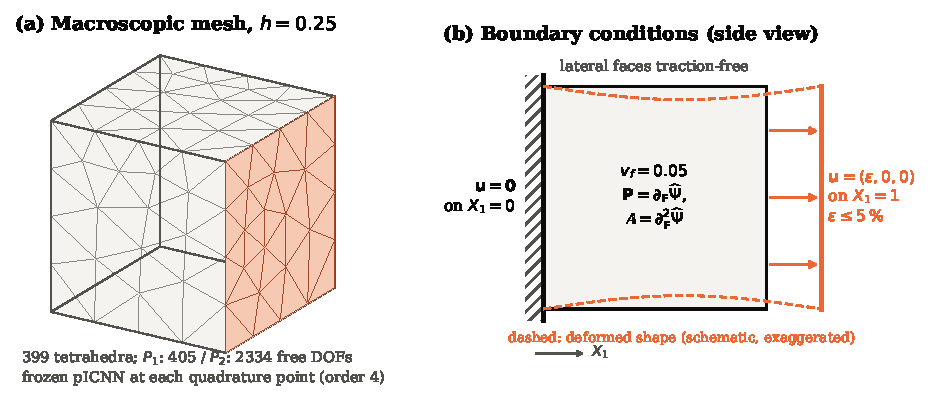
\includegraphics[width=\textwidth]{fig_macro_setup.pdf}
\caption[Macroscopic finite-element model]{Macroscopic finite-element model. (a) Unit-cube mesh for $h=0.25$; the
loaded face $X_1=1$ is shaded. (b) Boundary conditions: face $X_1=0$ clamped, face
$X_1=1$ displaced by $(\varepsilon,0,0)$ with lateral motion suppressed, lateral faces
traction-free. The frozen pICNN supplies stress and tangent at every quadrature
point.}
\label{fig:macrosetup}
\end{figure}

{\small
\begin{xltabular}{\textwidth}{@{}p{3.6cm}X@{}}
\caption{Macroscale finite-element setup.}\label{tab:macrosetup}\\
\toprule
Item & Setting\\
\midrule
\endfirsthead
\caption[]{\emph{(continued)}}\\
\toprule
Item & Setting\\
\midrule
\endhead
\bottomrule
\endfoot
Domain and mesh & unit cube (Netgen OCC), unstructured tetrahedra, $h=0.25/0.20/0.16$ with 399 / 648 / 1818 elements\\
Elements & vector Lagrange $P_1$ (405 / 642 / 1356 DOFs) or $P_2$ (2334 / 3759 / 8928 DOFs); displacement only\\
Quadrature & integration order 4 (46 points per tetrahedron; 18\,354 points at $h=0.25$), identical for $\bm R$, $\bm K$ and the material data\\
Material & frozen pICNN at $\vfrac=0.05$, evaluated at every quadrature point\\
Boundary conditions & $\bm u=\bm 0$ on $x=0$; $\bm u=(\varepsilon,0,0)$ on $x=1$; lateral faces traction-free\\
Loading & $\varepsilon=5\,\%$ in 100 increments ($P_1$); $0.5\,\%$ / $1\,\%$ in 10 / 20 increments ($P_2$)\\
Nonlinear solver & Newton with energy line search, secant predictor, spectral shift; tolerance $10^{-8}$\\
Linear solver & sparse direct factorization (UMFPACK)\\
\end{xltabular}
}

